\documentclass{article}
\usepackage{graphicx}
\usepackage{float}

\title{IdentiFisher: \\ User Guide \\}



\author{
\Large McDonald, Christopher\\
\texttt{1312456} \\ \\
\Large Guo, Tian\\
\texttt{1327833} \\ \\
\Large Murray, Shandelle\\
\texttt{1303109} \\ \\
\Large Cheung, Ocean\\
\texttt{1316057} \\
}

\vfill
\date{\today}

\begin{document}
\maketitle

\newpage
\tableofcontents
\vfill
\noindent \\


\pagebreak
\section{Introduction}

\subsection{Purpose of Application}


\subsection{Developers}
The software system will be named hereafter as IdentiFisher, which is an Android application.
This system will be a utility application for anyone who fishes, either recreationally or
competivitely. It will service beginner to experienced fishers. Identifisher will allow
the user to give information about a recently caught fish and help to identify what type
of fish it is. From there, it can collect data and track which types of fish are caught where. The aim is to
build a global logging system that will provide percentage catch rates by lake,
educate young, novice fishers, and integrate technology into a relatively non-technological field.


\section{Instruction}
This section will discuss the layout of each page of the application and the respective functions.
Walkthrough of how to complete a task will also be presented.
\subsection{Main Page}
The main page controls the display of other pages and their respective functions. The user may navigate to the
appropriate page from the main page based on what function is needed. \\
\begin{figure}[H]
	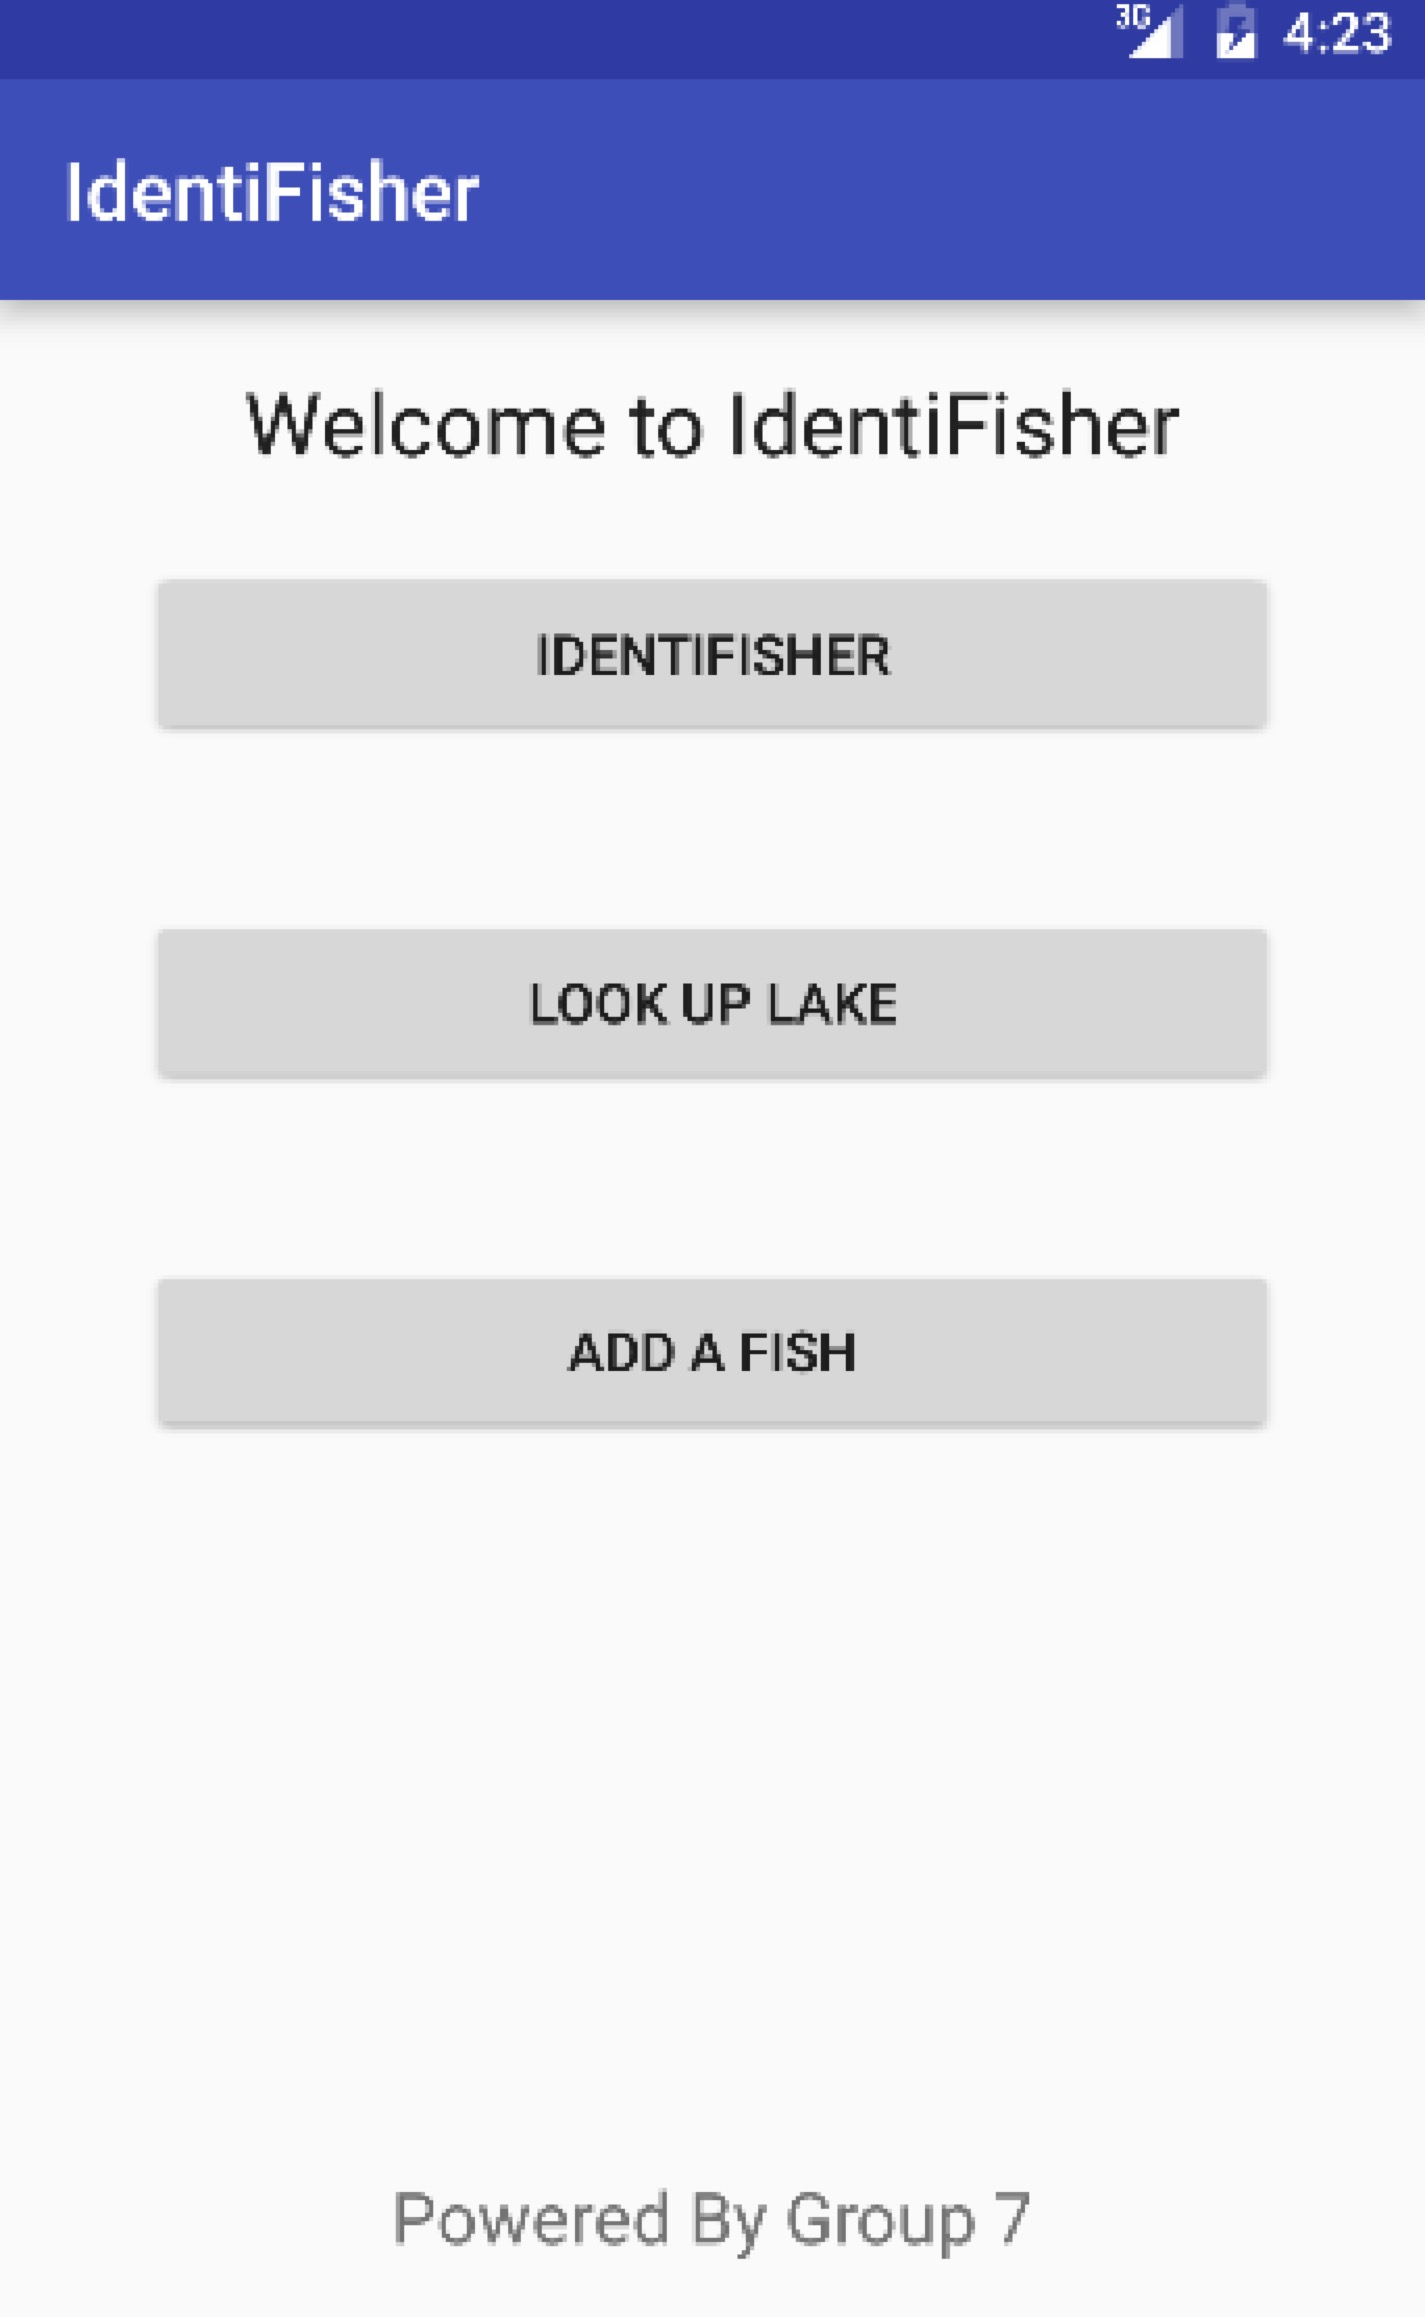
\includegraphics[scale=0.16]{Mainpage.png}
	\caption{Main page of IdentiFisher Application}
\end{figure}
The main page has the name of the application and the welcome message at the top of the screen. There are three
buttons that when pressed will navigate to a different page. The "IDENTIFISHER" button will take the user to a different page
where the user will select different properties of a fish to identify. The "LOOK UP LAKE" button will navigate to a page where the
user may search up a lake near a certain location to find the possible list of fish in the area. The "ADD A FISH" button will navigate
to a page where the user may add a fish with a location of fish found to the database of the app.\\
\subsection{IDENTIFISHER page}
The IDENTIFISHER page displays an instruction message at the top of the page: "Please enter the following criteria". There are three
drop down menus for colour, pattern, and shape of the fish respectively. There is a "IDENTIFY!" button underneath that the user can
start the identification when the correct properties are selected.


\newpage
\listoffigures

\end{document}
